% Page formatting
\documentclass[12pt]{article}
\usepackage[margin=1in]{geometry}
\usepackage[document]{ragged2e}

% Enumerations
\usepackage{enumitem}

% Colored box headings
\usepackage{xcolor}
\usepackage[explicit]{titlesec}

% Fonts
\usepackage{tgbonum}
\usepackage{avant}

% Figures
\usepackage{graphicx}
\usepackage[font={bf,sf,footnotesize},justification=justified,singlelinecheck=false]{caption}

% Debug
%\usepackage{showframe}



% Section colorings
\definecolor{sectioncolor}{HTML}{3399ff} 
\definecolor{subsectioncolor}{HTML}{ff9600} 

% Title formatting
\newcommand{\sectionheaderfmt}[1]{%
    \sffamily\bfseries\strut\color{white}#1
}

% Under-Title boxes boxes
\newcommand{\titlebox}[2]{%
    \colorbox{#1}{%
        \sectionheaderfmt{#2}%
}}

% Section boxes
\newcommand{\sectionbox}[2]{%
    \colorbox{#1}{%
        \parbox{\dimexpr\textwidth-6pt}{% 6pt is a Hack lol
            \sectionheaderfmt{#2}%
}}}

\titleformat{\section}{}{}{0pt}{%
    \sectionbox{sectioncolor}{\Large#1}%
}

\titleformat{\subsection}{}{}{0pt}{%
    \sectionbox{subsectioncolor}{\large#1}%
}

\begin{document}

%% Title page %%
\noindent
\titlebox{sectioncolor}{\large An Overview of the TLS Handshaking Protocol\hspace{5em}}

\medskip
\noindent
\titlebox{sectioncolor}{\large\today}

\medskip
\noindent
\titlebox{sectioncolor}{\large Duncan Freeman}

% No page numbering on first page
\thispagestyle{empty}

\newpage

%% Table of contents %%

\pagenumbering{roman}
\setcounter{page}{2}

\sffamily \tableofcontents \rmfamily

\newpage
%% List of figures %%

\sffamily \textbf{\listoffigures} \rmfamily

\newpage

%% Start of document %%

\pagenumbering{arabic}

\section{Introduction}
Transport Layer Security (TLS) is a protocol that facilitates privacy and authentication of messages (RFC 5246, 1). This document provides an overview of the TLS handshake subprocedure. This document does not cover implementation details, message transport, or specific ciphers. This document is arranged as follows: First, background information on TLS will be provided, followed by the two stages of the handshake procedure: Method Agreement, and Key Exchange \& Authentication. The conclusion will describe the utilization of the secure channel that the handshake establishes. 

\section{Background information}
TLS is a protocol used to secure private and untampered communications on the web (RFC 5246, 6, 78). For example, HTTPS is the original HTTP (HyperText Transfer Protocol) transmitted over a TLS transport instead of TCP (HTTP over TLS, 1). TLS is not a specific cipher or encryption method in itself; it is a standard container format that facilitates the use of a set of existing encryption methods (RFC 8446, 7).

\section{The TLS handshaking protocol}
First, a protocol version, cipher suite, and compression method is established. Then, keys are exchanged and digital certificates are verified.

\subsection{Stage I: Method agreement}

The client presents an array of protocol versions and ciphers it is willing to use, and the server selects one in response. Optionally, the pair may resume a prior session instead.

\begin{figure}[ht]
    \hspace{0.75cm}
    \begin{minipage}[c]{0.53\textwidth}
        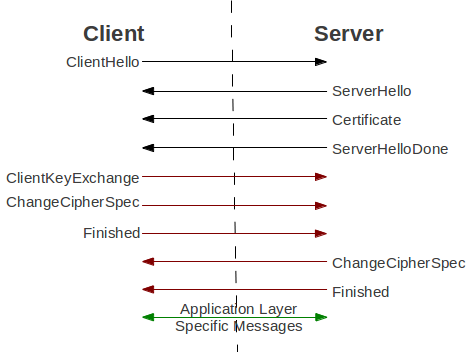
\includegraphics[width=\textwidth]{tls_protocol.png}
    \end{minipage}
    \begin{minipage}[c]{0.3\textwidth}
        \caption{TLS Handshake}%
        \label{Handshake}%
        \sffamily\footnotesize The TLS Handshake procedure is composed of a small number of negotiating messages that together form the configuration of the resultant message layer.
        \scriptsize\textcopyright\rmfamily\textit{Carnegie Mellon University 2012}
    \end{minipage}
\end{figure}

\begin{enumerate}[rightmargin=1cm]
    \item The client begins the conversation by sending a ‘ClientHello’ message (See Figure \ref{Handshake}), which contains information about what protocols it is capable of communicating over (RFC 8446, 12, RFC 5246, 34). The message includes the specific version of TLS that is intended to be used, encryption schemes the client supports, and compression methods available (RFC 8446, 12, RFC 5246, 34). Because encryption has not been established at this stage, this message is unencrypted; a MitM (Man-in-the-Middle) attack could be used to weaken the protocol by selecting for older versions of TLS or specific broken ciphers (RFC 5246, 34, 97). It is the responsibility of the applications using TLS to ensure that they do not allow communication over outdated protocols deemed insecure (RFC 5246, 34). Newer versions of TLS help to mitigate these attacks (See step 3).
    \item Optionally, the client sends a specialized ‘Resume’ message that describes a previous connection from which encryption and protocol parameters are to be reused (RFC 5246, 36, RFC 8446, 39). Following this message, no further authentication is needed for the session, and communication can begin immediately (RFC 5246, 35, 36). This can help to decrease the overhead of TLS in contexts where several concurrent or successive connections are established (RFC 8446, 74).
    \item The server picks from the protocol versions, ciphers, and compression methods offered by the client and sends its choice for each. Among the choices given, the server always picks the safest available (RFC 5246, 41, 97). In TLS 1.3, if a MitM protocol downgrade attack is suspected, the server will attempt to expose it by sending the client some false info that signals that it actually supports a safer protocol and that communication should terminate (RFC 8446, 32). 
\end{enumerate}

\subsection{Stage II: Key exchange and authentication}
The server sends its certificate and key, and the client (having verified said certificate) sends its own key and optionally its certificate if requested.

\begin{figure}[ht]
    \hspace{0.75cm}
    \begin{minipage}[c]{0.45\textwidth}
        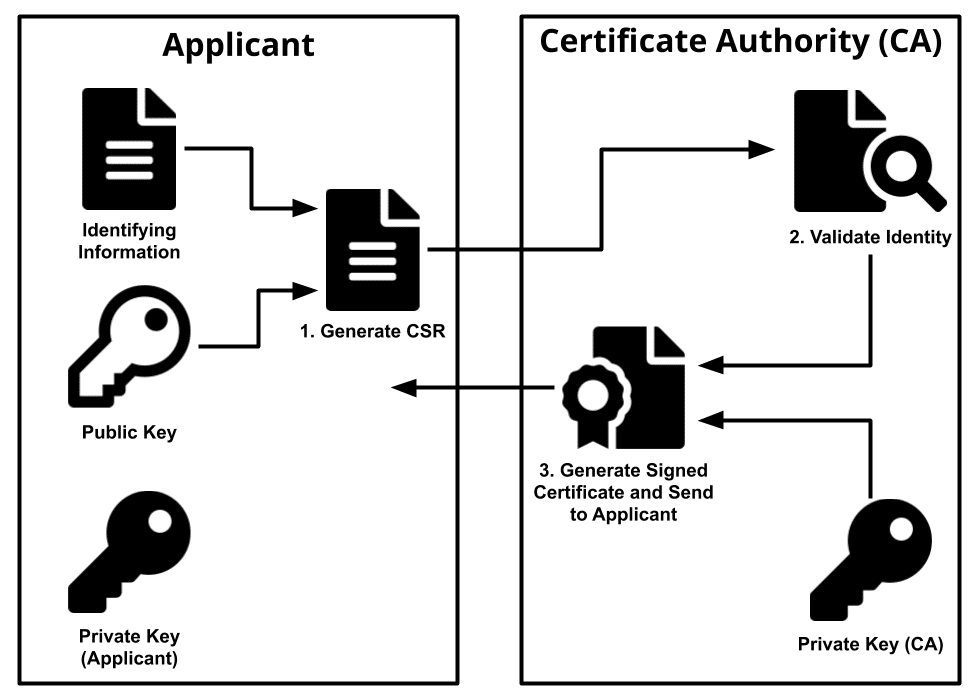
\includegraphics[width=\textwidth]{ca_diagram.png}
    \end{minipage}
    \begin{minipage}[c]{0.4\textwidth}
        \caption{Certificate Authority}
        \label{CA}%
        \sffamily\footnotesize The Certificate Authority validates the host's and/or client's public key using it's own private key, which protects the Applicant's connection against tampering.
        \scriptsize\textcopyright\rmfamily\textit{SSL.com 2019}
    \end{minipage}
\end{figure}

\begin{enumerate}[rightmargin=1cm]
    \item The server sends its certificate. The certificate proves mathematically that the public key contained in the following message originates from the server the client intended to connect to and that the server’s key was signed by a Certificate Authority (See Figure \ref{CA}) with which the client is familiar and trusts (What Are Certificate Authorities \& Trust Hierarchies?, 1). For a server to be trusted by clients, it must obtain a certificate from a trusted source with which to sign its key (GlobalSign, 1). It is the client’s responsibility to verify the server’s authenticity using this certificate (RFC 5246, 85).
    \item The server sends its key exchange message. This message contains the cryptographic information the client needs to compute a shared key with which to cipher and decipher information (RFC 5246, 50, RFC 8446, 31). This message may be omitted if there was enough information in the last transmission, to avoid overhead (RFC 5246, 50).
    \item Optionally, the server sends the client an authentication request (RFC 5246, 35, RFC 8446, 12). This request is an additional security measure requiring trust on the client side, but does incur overhead in the form of another message from the client side (RFC 8446, 12).
    \item The client sends its key exchange message. This message contains cryptographic information the server needs to compute a shared key with which to cipher and decipher information (RFC 5246, 35, 57). In TLS 1.3, all extra or nonstandard handshake communications following this are encrypted with the agreed-upon protocol for additional security (RFC 8446, 8). Barring any custom requirements, the handshake is over and the private channel is now ready for use (RFC 8446, 8).
\end{enumerate}

\section{Conclusion}
Following the success of the above procedure, the TLS connection is now initialized and ready for messaging over the TLS record protocol (RFC 8446, 71). Application-level protocols such as FTP, HTTP, SMTP and others may then utilize the record protocol to send messages transparently as if using the underlying TCP stream, but with the guarantee of encryption and authentication initialized by the handshake procedure (RFC 5246, 78).

\newpage

\section{Works cited}
\begin{description}[leftmargin=!,itemindent=-15pt]
    \item ``HTTP Over TLS.'' IETF Tools, May 2000. %https://tools.ietf.org/html/rfc2818.
    \item ``What Are Certificate Authorities \& Trust Hierarchies?'' What is a Certificate Authority? Globalsign. Accessed November 14, 2019. %https://www.globalsign.com/en/ssl-information-center/what-are-certification-authorities-trust-hierarchies/.
    \item ``The Transport Layer Security (TLS) Protocol Version 1.3.'' IETF Tools. IETF, August 2018. %https://tools.ietf.org/html/rfc8446. 
    \item ``The Transport Layer Security (TLS) Protocol Version 1.2.'' IETF Tools. IETF, August 2008. %https://tools.ietf.org/html/rfc5246.
\end{description}

\newpage

\section{Bibliography}

%https://www.ssl.com/faqs/what-is-a-certificate-authority/
%http://www.cs.cmu.edu/~mmaass/tpm_tls/report.html

\end{document}
